\pdfoutput=1
\documentclass[11pt]{article}
\usepackage{eacl2023}
\usepackage{times}
\usepackage{latexsym}
\usepackage[T1]{fontenc}
\usepackage[utf8]{inputenc}
\usepackage{microtype}
\usepackage{graphicx}
\usepackage{booktabs}
\usepackage{url}
\usepackage{placeins}
\usepackage{array}
\usepackage{amsmath}
\usepackage{enumitem}
\setlist[itemize]{noitemsep,topsep=2pt,parsep=0pt,partopsep=0pt}

\title{Bias-Aware Indic Spoken Language Identification}

\author{Project Team \\
Saarland University \\
\texttt{spoken-language-identification}}

\begin{document}
\maketitle
\nocite{pytorchaudioaugtutorial}

\begin{abstract}
This report studies Indic spoken language identification on \texttt{badrex/nnti-dataset-full}. We reproduce the baseline direction and improve a strong mHuBERT reference through tuning (0.4676 $\rightarrow$ 0.5270 accuracy). We then evaluate multiple speaker-bias mitigation variants and find that model-based adversarial training (DANN) gives the best final result: 0.5576 accuracy and 0.5426 macro-F1. We analyze bias source, mitigation success, confusion patterns, and last-layer t-SNE behavior. Results show clear bias reduction and weak-class recovery, but not complete removal of speaker information.
\end{abstract}

\section*{1 Introduction}
This project studies spoken language identification under strong speaker-shift conditions. The key challenge is that the model must learn language cues from a limited set of training speakers and generalize to fully unseen validation speakers.

Implementation uses PyTorch \citep{paszke2019pytorch}, torchaudio augmentation practice from the PyTorch Audio tutorial, Hugging Face Transformers/Datasets \citep{wolf2020transformers}, scikit-learn \citep{pedregosa2011scikit}, Matplotlib \citep{hunter2007matplotlib}, MMS \citep{pratap2023mms}, wav2vec2 \citep{baevski2020wav2vec2}, HuBERT \citep{hsu2021hubert}, DANN \citep{ganin2016dann}, and t-SNE \citep{maaten2008tsne}.

\section*{2 Dataset}
We use \texttt{badrex/nnti-dataset-full} \citep{badr2026dataset}. Core split statistics:
\begin{itemize}
    \item Languages: 22
    \item Train samples: 8689
    \item Validation samples: 3300
    \item Train unique speakers: 110
    \item Validation unique speakers: 681
    \item Train/validation speaker overlap: 0
\end{itemize}

This is a strict unseen-speaker setting because all validation samples are from speakers absent in training.

\section*{3 experiments}
\subsection*{3.1 experimental setup (over all experientmental settings)}
To keep comparisons fair, we kept data split and seed fixed and changed only intended components per run. Shared protocol:
\begin{itemize}
    \item Fixed split: same train/validation files across runs.
    \item Fixed seed: 42.
    \item Best-checkpoint loading enabled (\texttt{load\_best\_model\_at\_end=True}).
    \item Same diagnostics family: per-language accuracy, confusion matrix, speaker diagnostics.
\end{itemize}

\subsection*{3.2 eval metrics (overall eval metrics used)}
We report:
\begin{itemize}
    \item Global metrics: validation accuracy, macro-F1, eval loss.
    \item Class-level metric: per-language validation accuracy.
    \item Error structure: off-diagonal confusion pairs from confusion matrix.
    \item Speaker diagnostics: overlap count and unseen-speaker accuracy.
    \item Representation diagnostics: last-layer t-SNE (where artifacts are available).
\end{itemize}

For final ranking in speaker-bias mitigation, macro-F1 is prioritized with accuracy as a guardrail.

\section*{4 Baseline system and improvements}
\subsection*{4.1 Methods}
The baseline-improvement pipeline followed two stages:
\begin{itemize}
    \item \textbf{Baseline direction reproduction}: supervised fine-tuning from assignment baseline family (MMS-300m setup).
    \item \textbf{Improvement stage}: backbone and hyperparameter improvements leading to tuned mHuBERT reference.
\end{itemize}

In the improvement stage, we focused on reproducible tuning rather than architecture redesign: learning-rate/schedule tuning, checkpoint-selection strategy, and stable training controls. Reporting these hyperparameter-level changes is useful because final quality depends strongly on training setup, not only on backbone choice.

The main hyperparameter settings reported for this baseline-improvement stage are: target learning rate (around \(1\times10^{-5}\) with warmup schedule), effective batch control (per-device batch size with gradient accumulation), checkpointing policy (\texttt{load\_best\_model\_at\_end=True}), model-selection metric (accuracy for the tuned no-mitigation reference), and evaluation/save cadence during training. These settings are part of the method because they materially changed final quality.

The tuned mHuBERT reference became the no-mitigation control for speaker-bias mitigation experiments.

\subsection*{4.2 experiments}
We executed three experimental checkpoints in sequence: (i) baseline direction using MMS-300m reference performance from the assignment, (ii) untuned mHuBERT run, and (iii) tuned mHuBERT run. This sequence isolates the effect of model choice and tuning quality before any mitigation logic is added.

\begin{table}[h]
\centering
\small
\setlength{\tabcolsep}{4pt}
\begin{tabular}{@{}p{0.46\columnwidth}rrr@{}}
\toprule
Run & Acc & Macro-F1 & Eval Loss \\
\midrule
Assignment baseline (MMS-300m) & 0.3196 & -- & -- \\
mHuBERT untuned & 0.4676 & 0.4142 & 2.2854 \\
mHuBERT tuned & \textbf{0.5270} & \textbf{0.4748} & \textbf{2.1629} \\
\bottomrule
\end{tabular}
\caption{Baseline and improvement experiment summary.}
\label{tab:task1_summary}
\end{table}
\FloatBarrier

\subsection*{4.3 results}
In baseline-direction reproduction, the provided MMS-300m baseline is 31.96\% top-1 accuracy. The untuned mHuBERT run already exceeds that level (0.4676), and tuned mHuBERT further improves to 0.5270 accuracy and 0.4748 macro-F1. Relative to untuned mHuBERT, tuning adds +0.0594 accuracy and +0.0607 macro-F1. This tuned run is the direct control for all mitigation comparisons.

\section*{5 Speaker-Bias Mitigation}
\subsection*{5.1 Methods}
We used both data-centric and model-based mitigation.

\textbf{Data-centric mitigation:}
\begin{itemize}
    \item Mitigation 1: speed/noise augmentation ($p=0.30$, speed 0.97--1.03, noise std 0.0005--0.002).
    \item Mitigation 2: gentler speed/noise ($p=0.25$, speed 0.98--1.02, noise std 0.0005--0.0015) with macro-F1 checkpointing.
    \item Mitigation 3A: revert to M1 augmentation strength, macro-F1 checkpointing, denser eval/save cadence (100/100).
    \item Mitigation 3B: milder fallback from 3A ($p=0.28$, speed 0.975--1.025, noise std max 0.0018).
    \item Mitigation 4: all data-centric mix (speed/noise + pitch shift + spectral masking) with global augmentation gate and t-SNE export.
\end{itemize}

\textbf{Model-based mitigation (DANN):}
\begin{itemize}
    \item Architecture: shared encoder with two heads, one for language prediction and one adversarial head for speaker prediction.
    \item Training logic: a gradient reversal layer forces the encoder to reduce speaker-identifiable information while preserving language-discriminative features.
    \item Final DANN settings: \texttt{speaker\_loss\_weight=0.1}, \texttt{grl\_lambda=1.0}, lambda schedule enabled, speaker-head dropout 0.1.
    \item Run design: augmentation was disabled in the final DANN run to isolate the effect of adversarial mitigation from augmentation effects.
\end{itemize}

Encoder objective:
\[
\mathcal{L}_{enc} = \mathcal{L}_{lang} - \lambda \mathcal{L}_{speaker}.
\]

\subsection*{5.2 experiments}
We evaluated mitigation variants against the tuned no-mitigation reference on the same split and metrics. Table~\ref{tab:task2_summary} reports global quality, and Table~\ref{tab:mitigation_confusions} tracks high-impact confusion pairs across untuned, tuned, mitigation-1, and DANN runs.

\begin{table}[h]
\centering
\small
\setlength{\tabcolsep}{3pt}
\begin{tabular}{@{}p{0.47\columnwidth}rrr@{}}
\toprule
Run & Acc & Macro-F1 & Eval Loss \\
\midrule
Tuned ref (no mitigation) & 0.5270 & 0.4748 & 2.1629 \\
Mitigation 1 & 0.5388 & 0.4868 & 2.1504 \\
Mitigation 2 & 0.5279 & 0.4828 & 2.1385 \\
Mitigation 3A & 0.4979 & 0.4561 & 2.1884 \\
Mitigation 3B & 0.5276 & 0.4817 & 2.1456 \\
Mitigation 4 & 0.5115 & 0.4664 & 2.2127 \\
DANN (final improved) & \textbf{0.5576} & \textbf{0.5426} & \textbf{1.8815} \\
\bottomrule
\end{tabular}
\caption{Mitigation experiments (validation split).}
\label{tab:task2_summary}
\end{table}

\begin{table}[h]
\centering
\small
\setlength{\tabcolsep}{2.5pt}
\resizebox{\columnwidth}{!}{
\begin{tabular}{@{}lrrrr@{}}
\toprule
Pair & Untuned & Tuned & Mitigation 1 & DANN \\
\midrule
konkani$\rightarrow$marathi & 106 & 97 & 106 & 74 \\
sindhi$\rightarrow$punjabi & 79 & 103 & 102 & 14 \\
hindi$\rightarrow$urdu & 60 & 77 & 68 & 39 \\
dogri$\rightarrow$punjabi & 53 & 76 & 71 & 44 \\
bodo$\rightarrow$manipuri & 39 & 29 & 39 & 45 \\
odia$\rightarrow$bengali & 26 & 23 & 45 & 10 \\
santali$\rightarrow$bengali & 54 & 34 & 40 & 10 \\
\bottomrule
\end{tabular}
}
\caption{Confusion-pair counts across key runs (validation).}
\label{tab:mitigation_confusions}
\end{table}

\FloatBarrier

\subsection*{5.3 results}
Overall, DANN is the strongest mitigation result: +0.0306 accuracy and +0.0678 macro-F1 over tuned no-mitigation, and +0.0188 accuracy and +0.0558 macro-F1 over Mitigation 1. Data-centric methods were useful but sensitive to augmentation strength; Mitigation 1 was the best data-centric variant, while stronger mixed augmentation (Mitigation 4) underperformed.

Confusion behavior also improved for several high-impact pairs (Table~\ref{tab:mitigation_confusions}), especially \texttt{sindhi$\rightarrow$punjabi} and \texttt{hindi$\rightarrow$urdu}. Some pairs remain difficult (for example \texttt{konkani$\rightarrow$marathi}), so mitigation is strong but not complete.

Speaker-bias diagnostics support that these gains are not from speaker leakage: all key runs show \texttt{overlap\_speaker\_count=0} and no warnings, while unseen-speaker accuracy improves from 0.4676 (untuned) to 0.5576 (DANN). We also observe substantial recovery on historically weak classes, with weak-class mean accuracy increasing from 0.0227 (untuned) to 0.3547 (DANN).

\section*{6 analysis}
\subsection*{6.1 Bias Source and Learning Difficulty}
The bias source is limited speaker diversity in training (110 speakers over 22 languages) combined with a strict unseen-speaker validation set (681 speakers, 3300 validation samples). This creates a shortcut risk: during optimization, speaker timbre/prosody can become an easier signal than language-discriminative content.

Learning is difficult for two reasons. First, with few speakers per language, the encoder can partially fit speaker-correlated cues in train even when validation speakers are disjoint. Second, related-language pairs have overlapping acoustic/prosodic signatures, so weak classes remain under-separated.

Evidence from this project:
\begin{itemize}
    \item Untuned reference has near-zero classes (for example maithili 0.0000, konkani 0.0000, sindhi 0.0333).
    \item Baseline confusion mass concentrates in a few pairs (for example konkani$\rightarrow$marathi and sindhi$\rightarrow$punjabi).
    \item Validation is fully unseen-speaker (seen-speaker samples = 0, unseen-speaker samples = 3300), so weak performance cannot be explained by train/validation speaker overlap.
\end{itemize}

\subsection*{6.2 Mitigation Approach and Success Extent}
Our approach combines controlled data-centric variability and model-based adversarial de-biasing.
\begin{itemize}
    \item Data-centric mitigation (especially Mitigation 1) improves robustness by breaking fixed speaker-style dependence.
    \item DANN directly penalizes speaker-identifiable features in the shared encoder.
\end{itemize}

Measured outcome is strong but partial. Global gains are summarized in Table~\ref{tab:dann_impact}.

\begin{table}[h]
\centering
\small
\setlength{\tabcolsep}{4pt}
\begin{tabular}{@{}lrr@{}}
\toprule
Comparison & $\Delta$Acc & $\Delta$Macro-F1 \\
\midrule
Untuned $\rightarrow$ DANN & +0.0900 & +0.1284 \\
Tuned no-mitigation $\rightarrow$ DANN & +0.0306 & +0.0678 \\
Mitigation 1 $\rightarrow$ DANN & +0.0188 & +0.0558 \\
\bottomrule
\end{tabular}
\caption{Global impact of DANN versus reference runs.}
\label{tab:dann_impact}
\end{table}

Class-level behavior shows gains and tradeoffs: unseen-speaker accuracy improves from 0.4676 to 0.5576, weak-class mean rises from 0.0227 to 0.3547, and some previously strong classes still regress (for example nepali and punjabi vs Mitigation 1).

\subsection*{6.3 Confusion Patterns}
Most frequent confusions are:
\begin{itemize}
    \item \texttt{konkani$\rightarrow$marathi}
    \item \texttt{sindhi$\rightarrow$punjabi}
    \item \texttt{hindi$\rightarrow$urdu}
\end{itemize}

\begin{figure*}[!htbp]
    \centering
    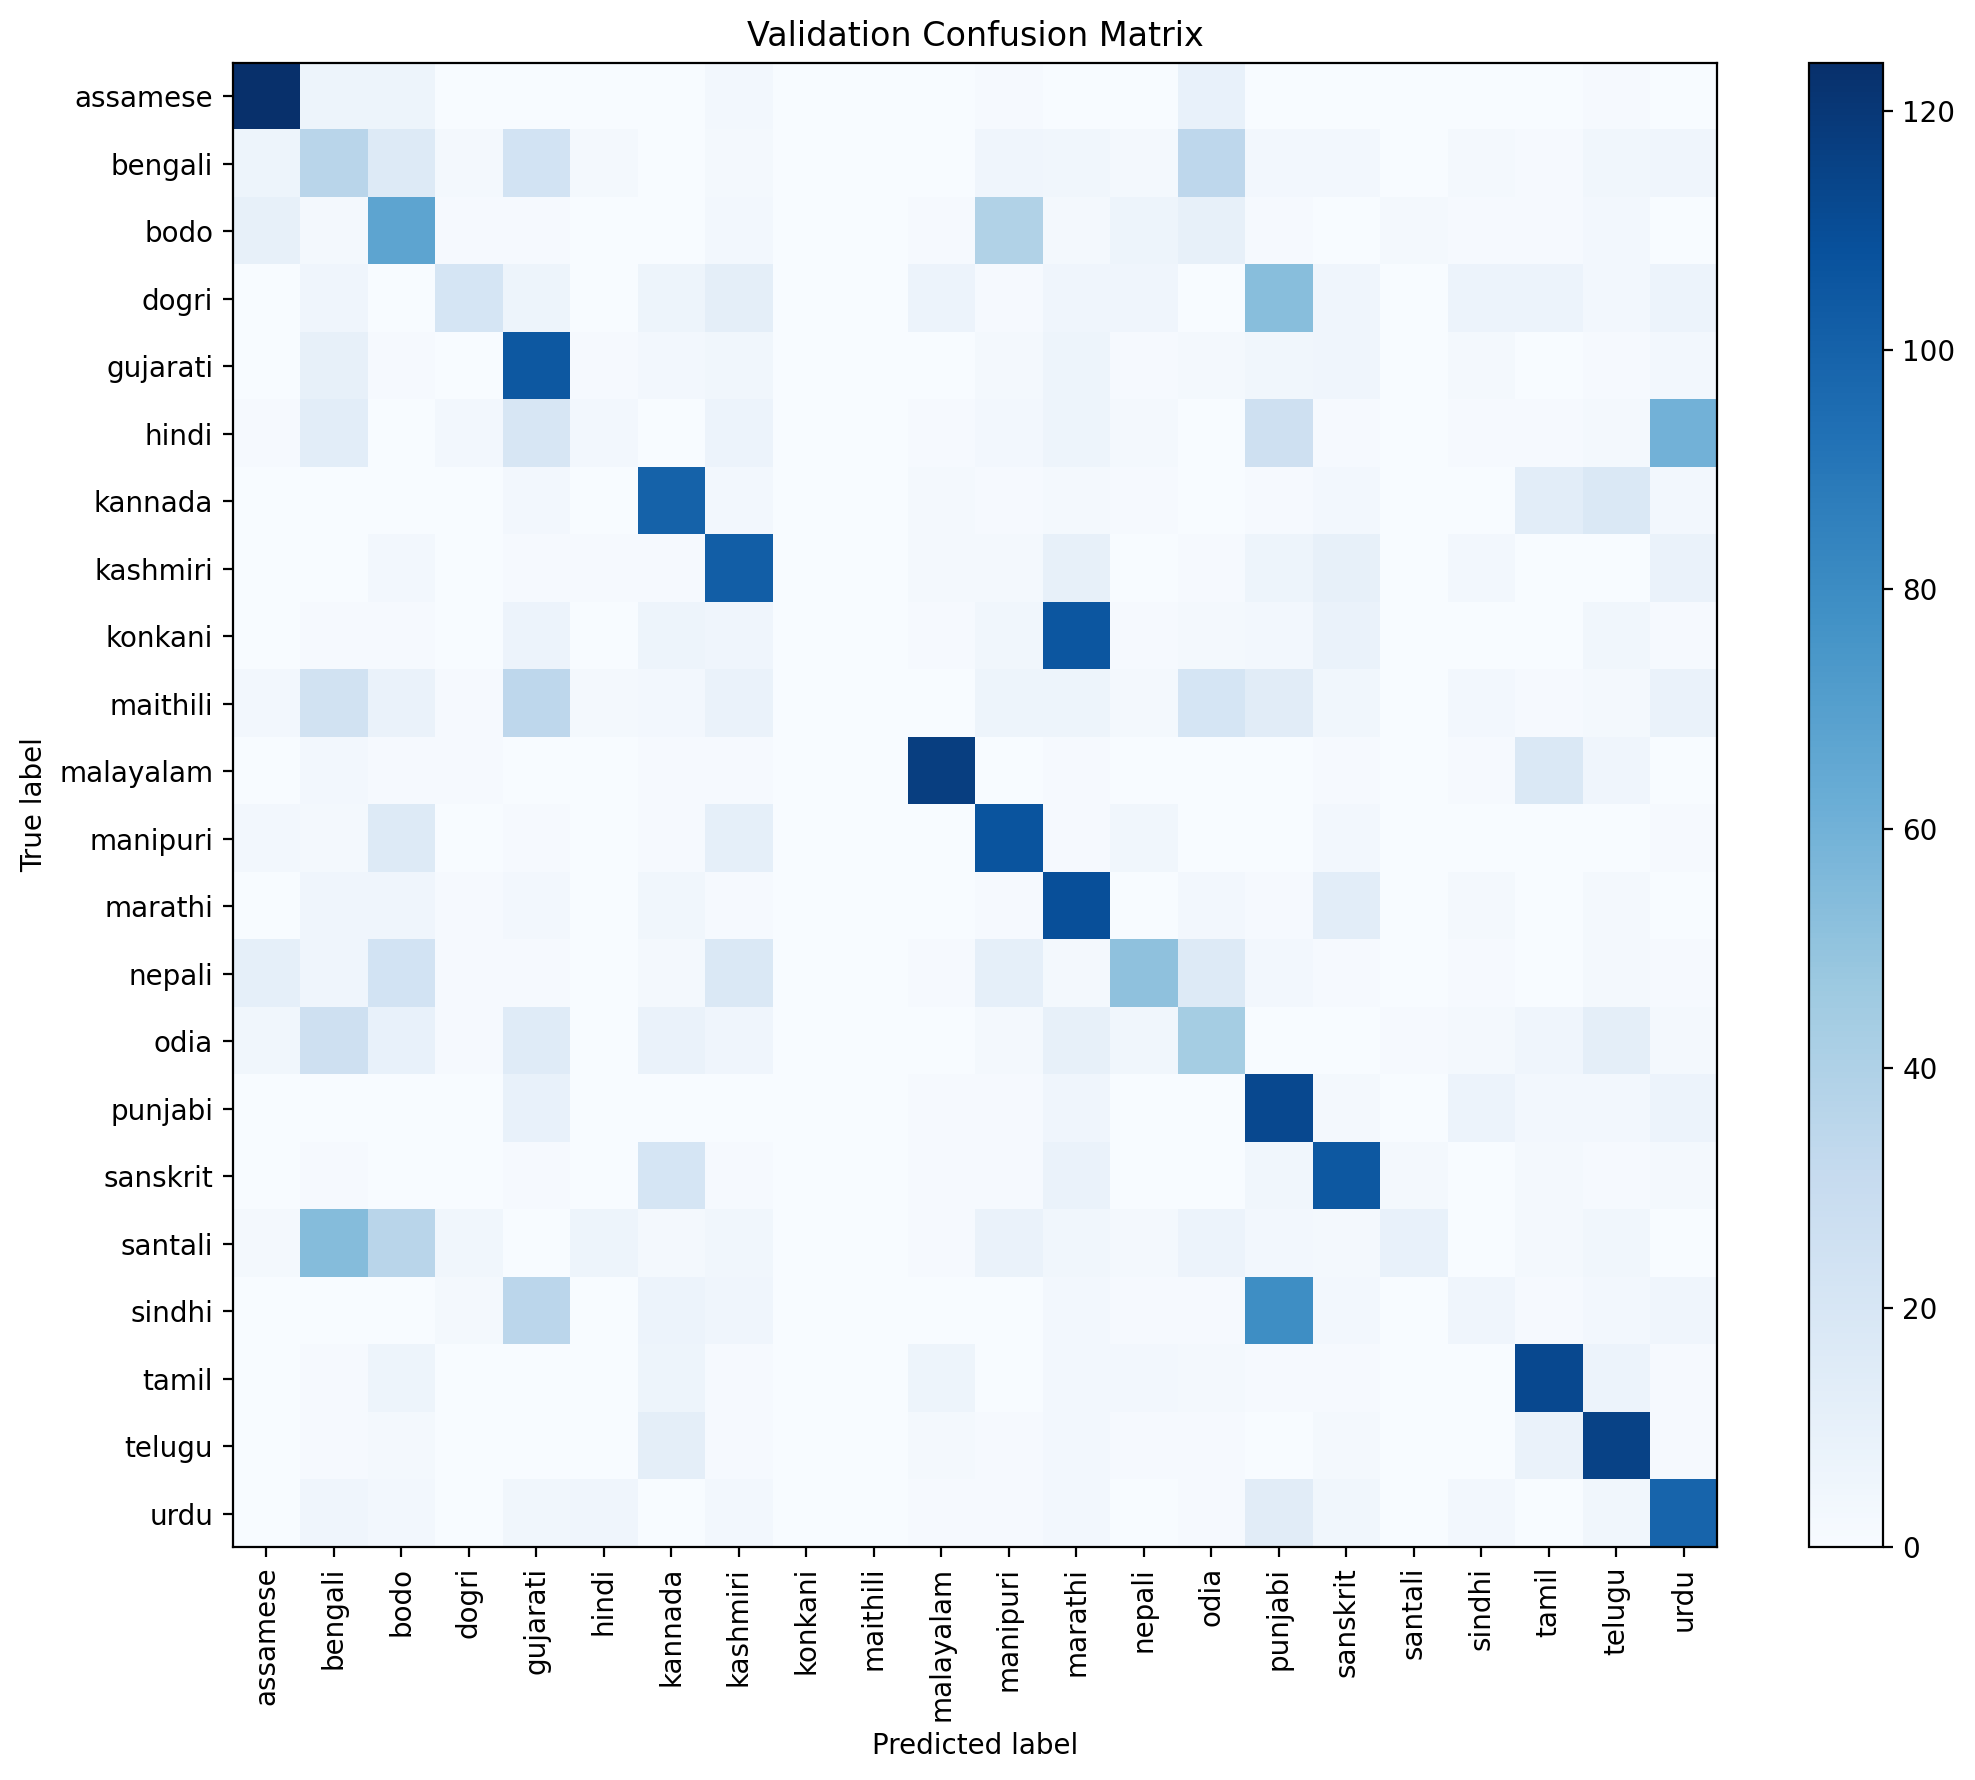
\includegraphics[width=0.31\textwidth]{figures/confusion_baseline_untuned.png}
    \hfill
    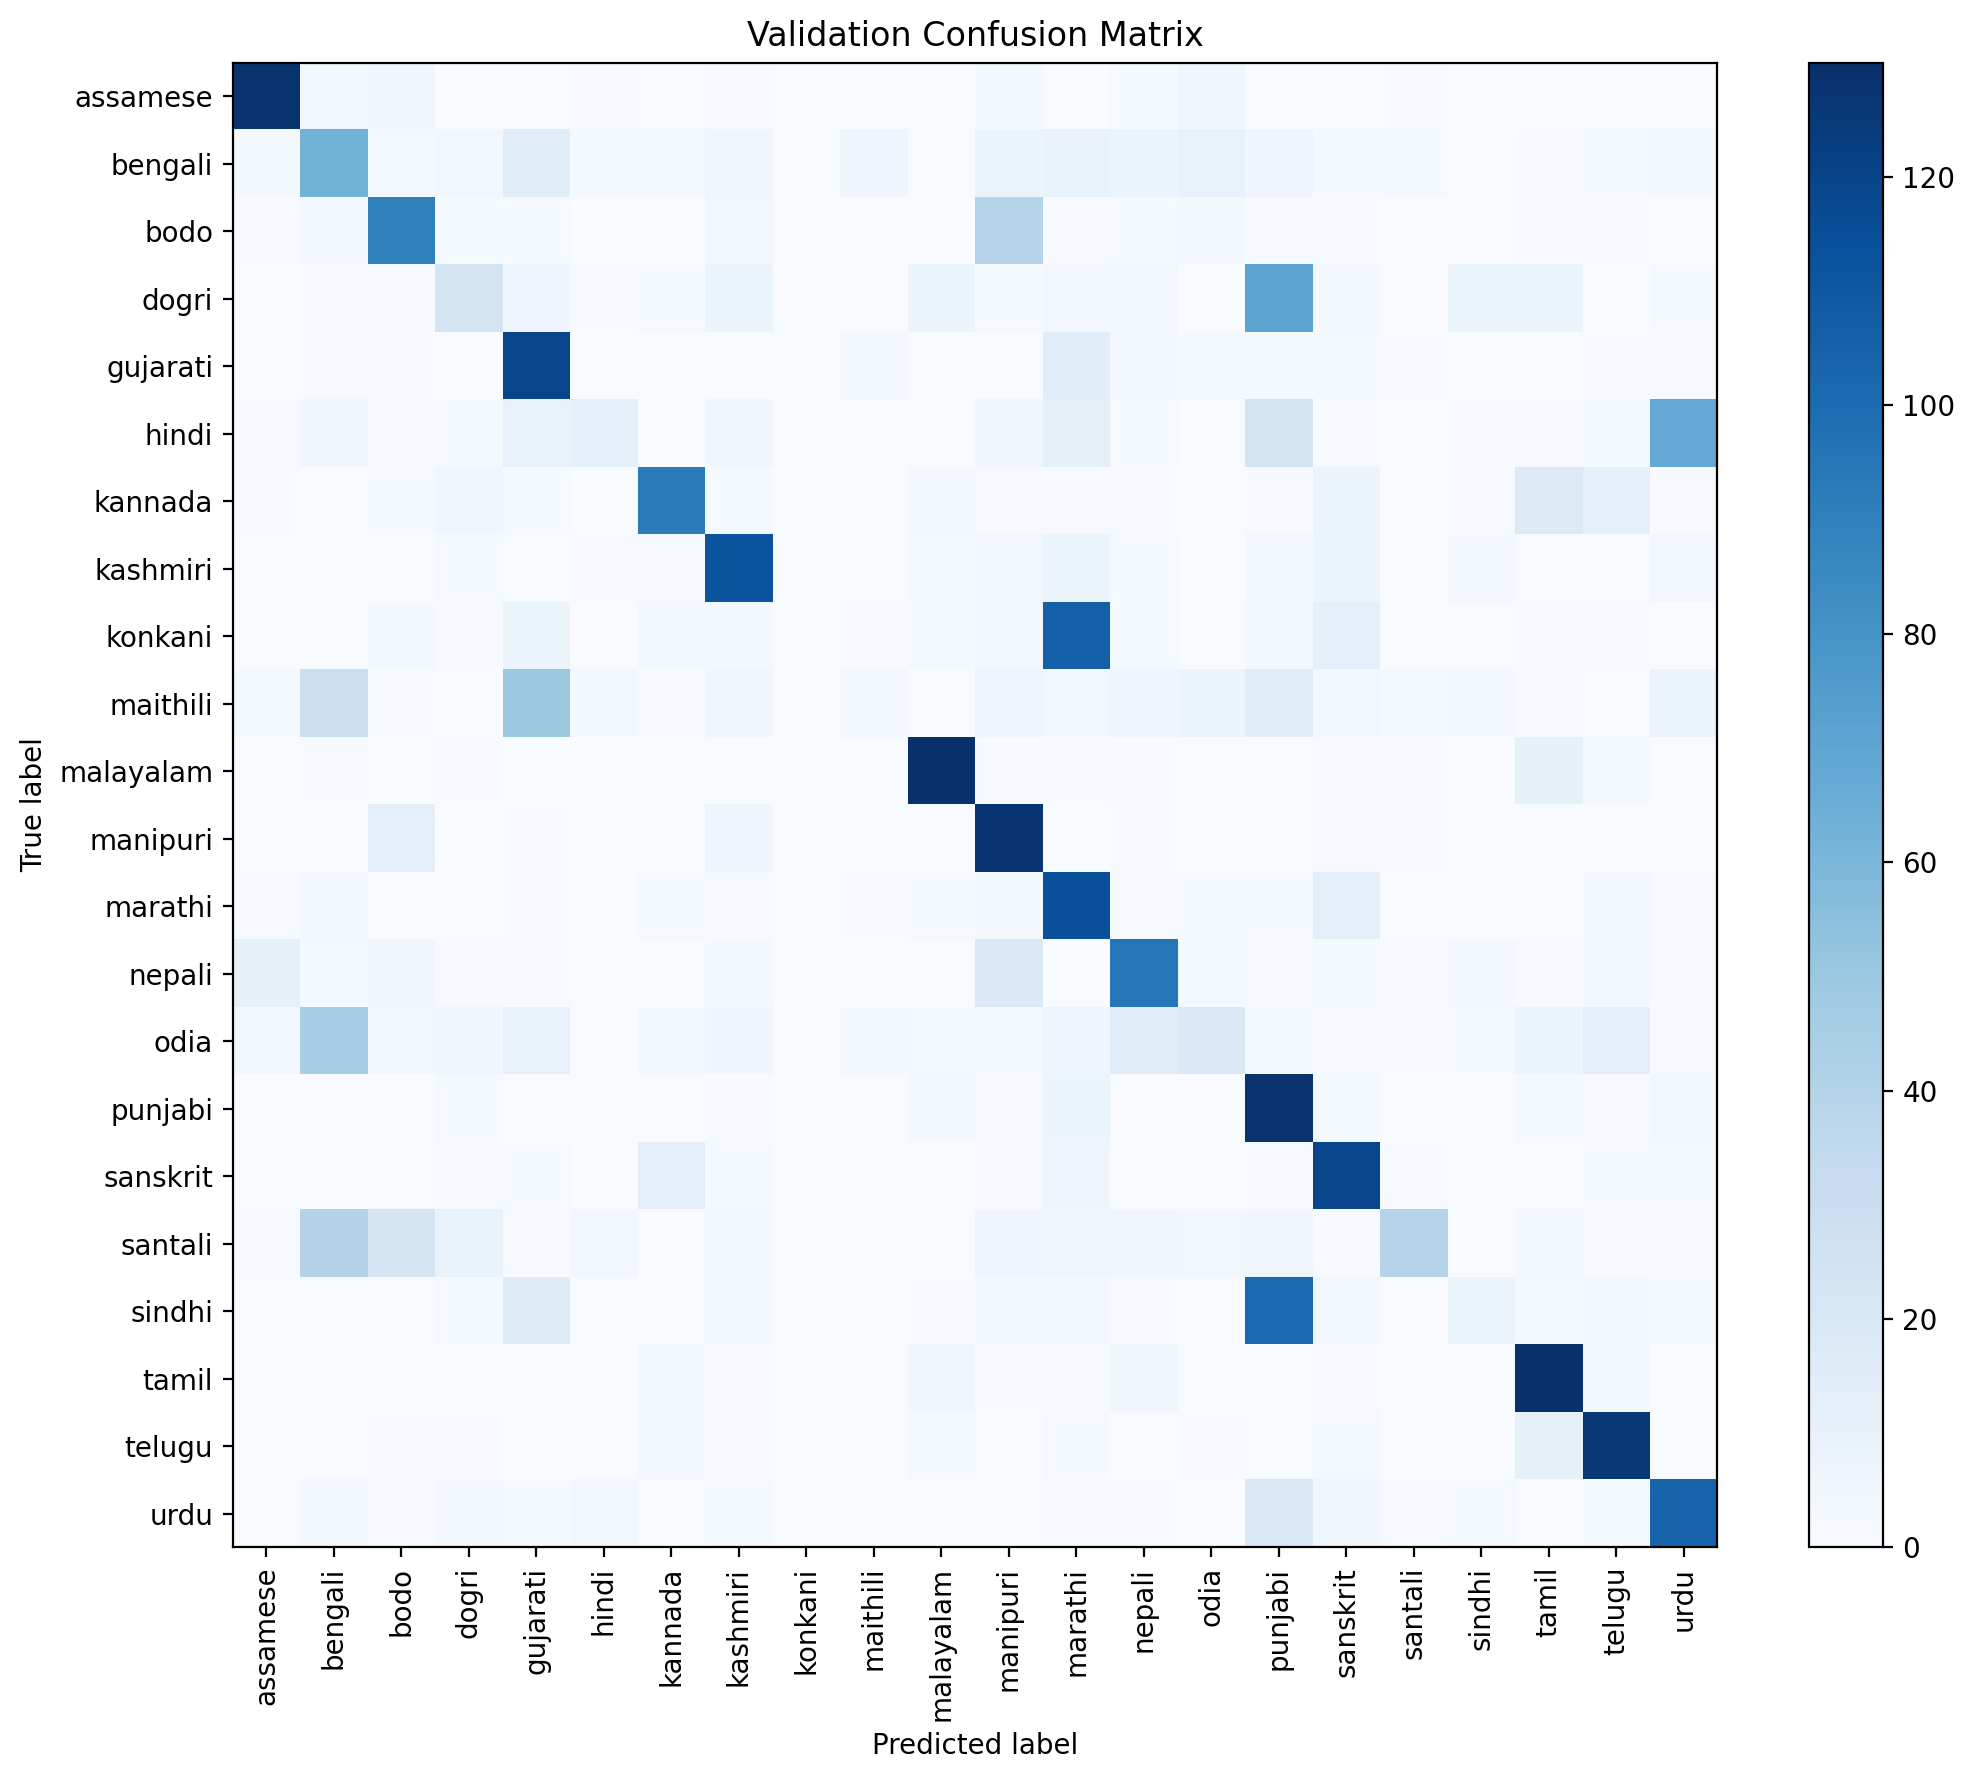
\includegraphics[width=0.31\textwidth]{figures/confusion_mitigation1.png}
    \hfill
    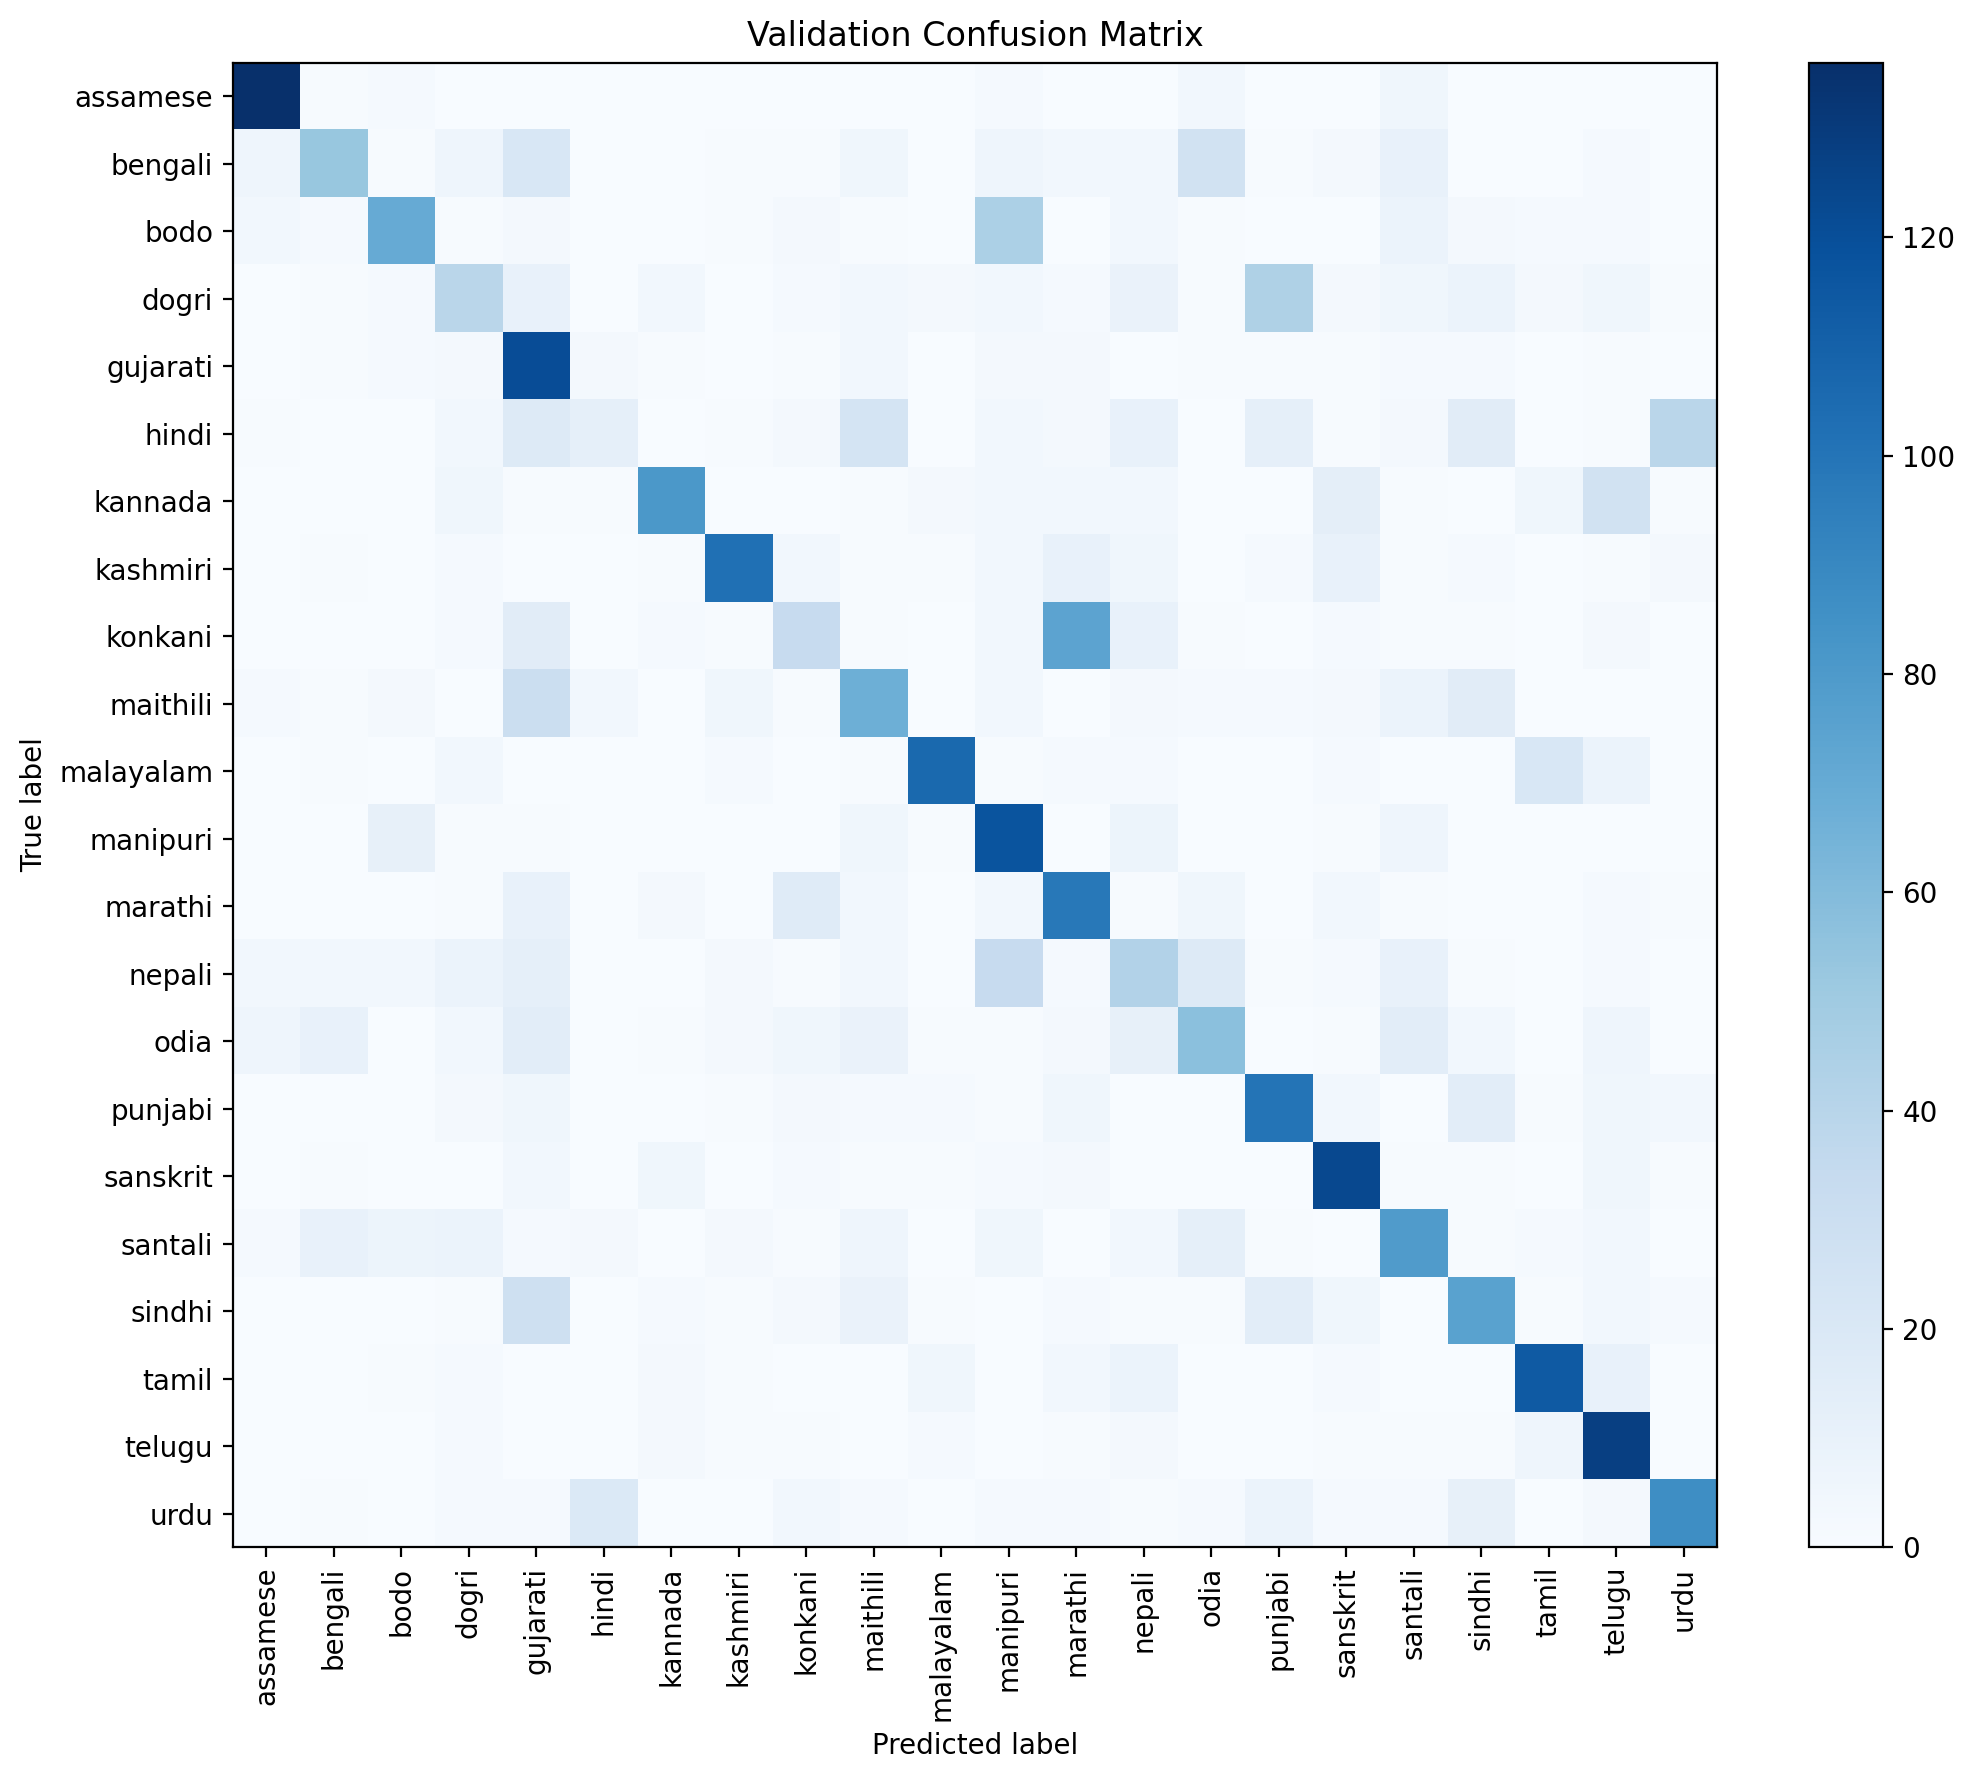
\includegraphics[width=0.31\textwidth]{figures/confusion_dann.png}
    \caption{Validation confusion matrices: untuned reference (left), Mitigation 1 (middle), DANN improved (right).}
    \label{fig:confusions}
\end{figure*}

These are plausible due to linguistic/acoustic proximity and insufficient class-separating cues in short utterances. As shown in Table~\ref{tab:mitigation_confusions}, DANN reduces several high-volume confusions, but not all.

Pattern-specific interpretation:
\begin{itemize}
    \item \texttt{hindi$\rightarrow$urdu}: high lexical and prosodic similarity in conversational speech.
    \item \texttt{konkani$\rightarrow$marathi}: regional/contact similarity and overlapping speaking styles.
    \item \texttt{sindhi$\rightarrow$punjabi}: difficult boundary under uneven class difficulty; strongly reduced by DANN (102 $\rightarrow$ 14 vs Mitigation 1).
    \item \texttt{odia$\rightarrow$bengali} and \texttt{santali$\rightarrow$bengali}: neighboring-language proximity; both reduced in DANN.
\end{itemize}

DANN improves multiple dominant confusions versus untuned baseline (\texttt{sindhi$\rightarrow$punjabi} 79$\rightarrow$14, \texttt{santali$\rightarrow$bengali} 54$\rightarrow$10, \texttt{odia$\rightarrow$bengali} 26$\rightarrow$10, \texttt{hindi$\rightarrow$urdu} 60$\rightarrow$39, \texttt{konkani$\rightarrow$marathi} 106$\rightarrow$74). At the same time, some alternative confusion channels increase (for example \texttt{bodo$\rightarrow$manipuri} 39$\rightarrow$45 and \texttt{nepali$\rightarrow$manipuri} 18$\rightarrow$33 when compared with Mitigation 1), showing that error redistribution still exists.

\subsection*{6.4 Representation Analysis (t-SNE)}
t-SNE is applied to last-layer validation embeddings. In local final artifacts, full t-SNE exports are available for DANN; untuned/tuned/Mitigation-1 t-SNE exports are not fully available in this branch snapshot.

For comparability, the analysis target setup is fixed (\texttt{max\_samples}=2200, \texttt{perplexity}=30, \texttt{seed}=42, \texttt{speaker\_top\_k}=12).

For DANN:
\begin{itemize}
    \item Silhouette (language): 0.0047
    \item Silhouette (speaker top-k): -0.0992
    \item kNN speaker purity@5: 0.3433
\end{itemize}

Interpretation: speaker structure is reduced but still present, so speaker identity is not fully removed from representations. The non-zero local speaker purity indicates residual speaker information in embedding neighborhoods, even after adversarial mitigation.

Because baseline/tuned/Mitigation-1 t-SNE point exports are missing in this local snapshot, we avoid overclaiming geometric comparison across all runs. However, combined with split diagnostics (overlap=0, no warnings) and unseen-speaker accuracy gains, DANN still shows better speaker-robust language behavior than earlier references.

\begin{figure}[t]
    \centering
    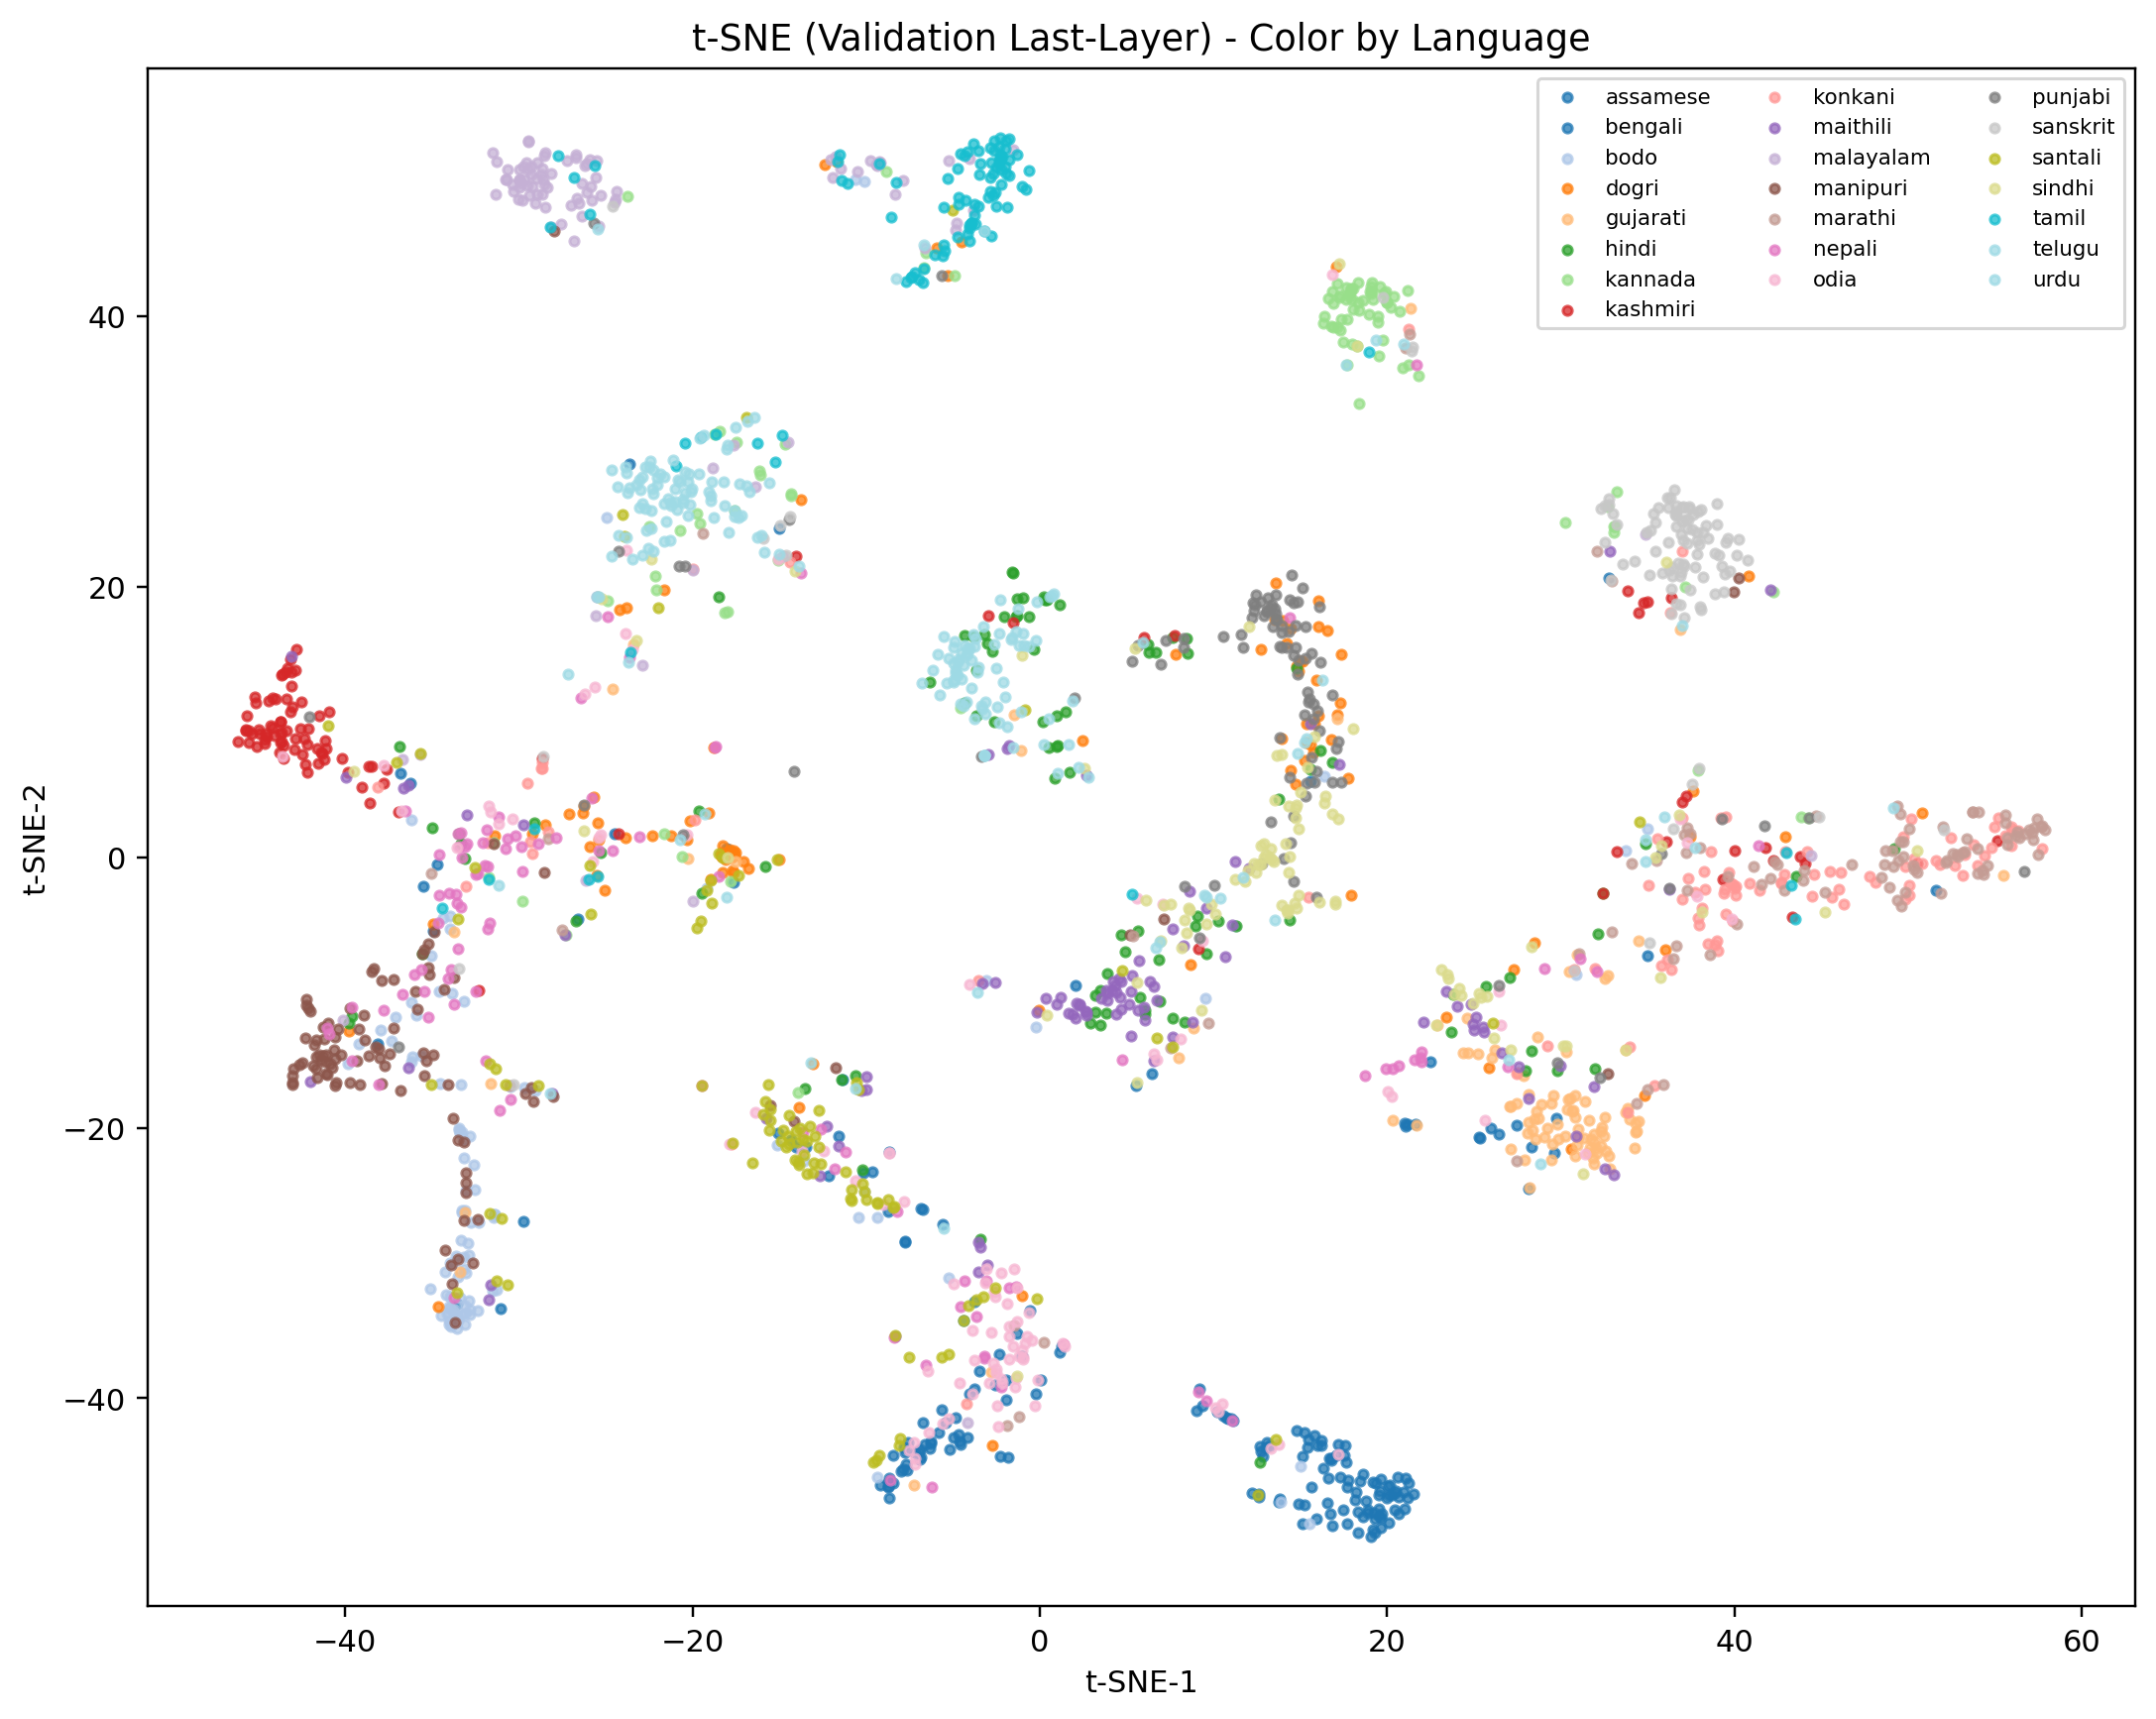
\includegraphics[width=0.48\linewidth]{figures/tsne_dann_by_language.png}
    \hfill
    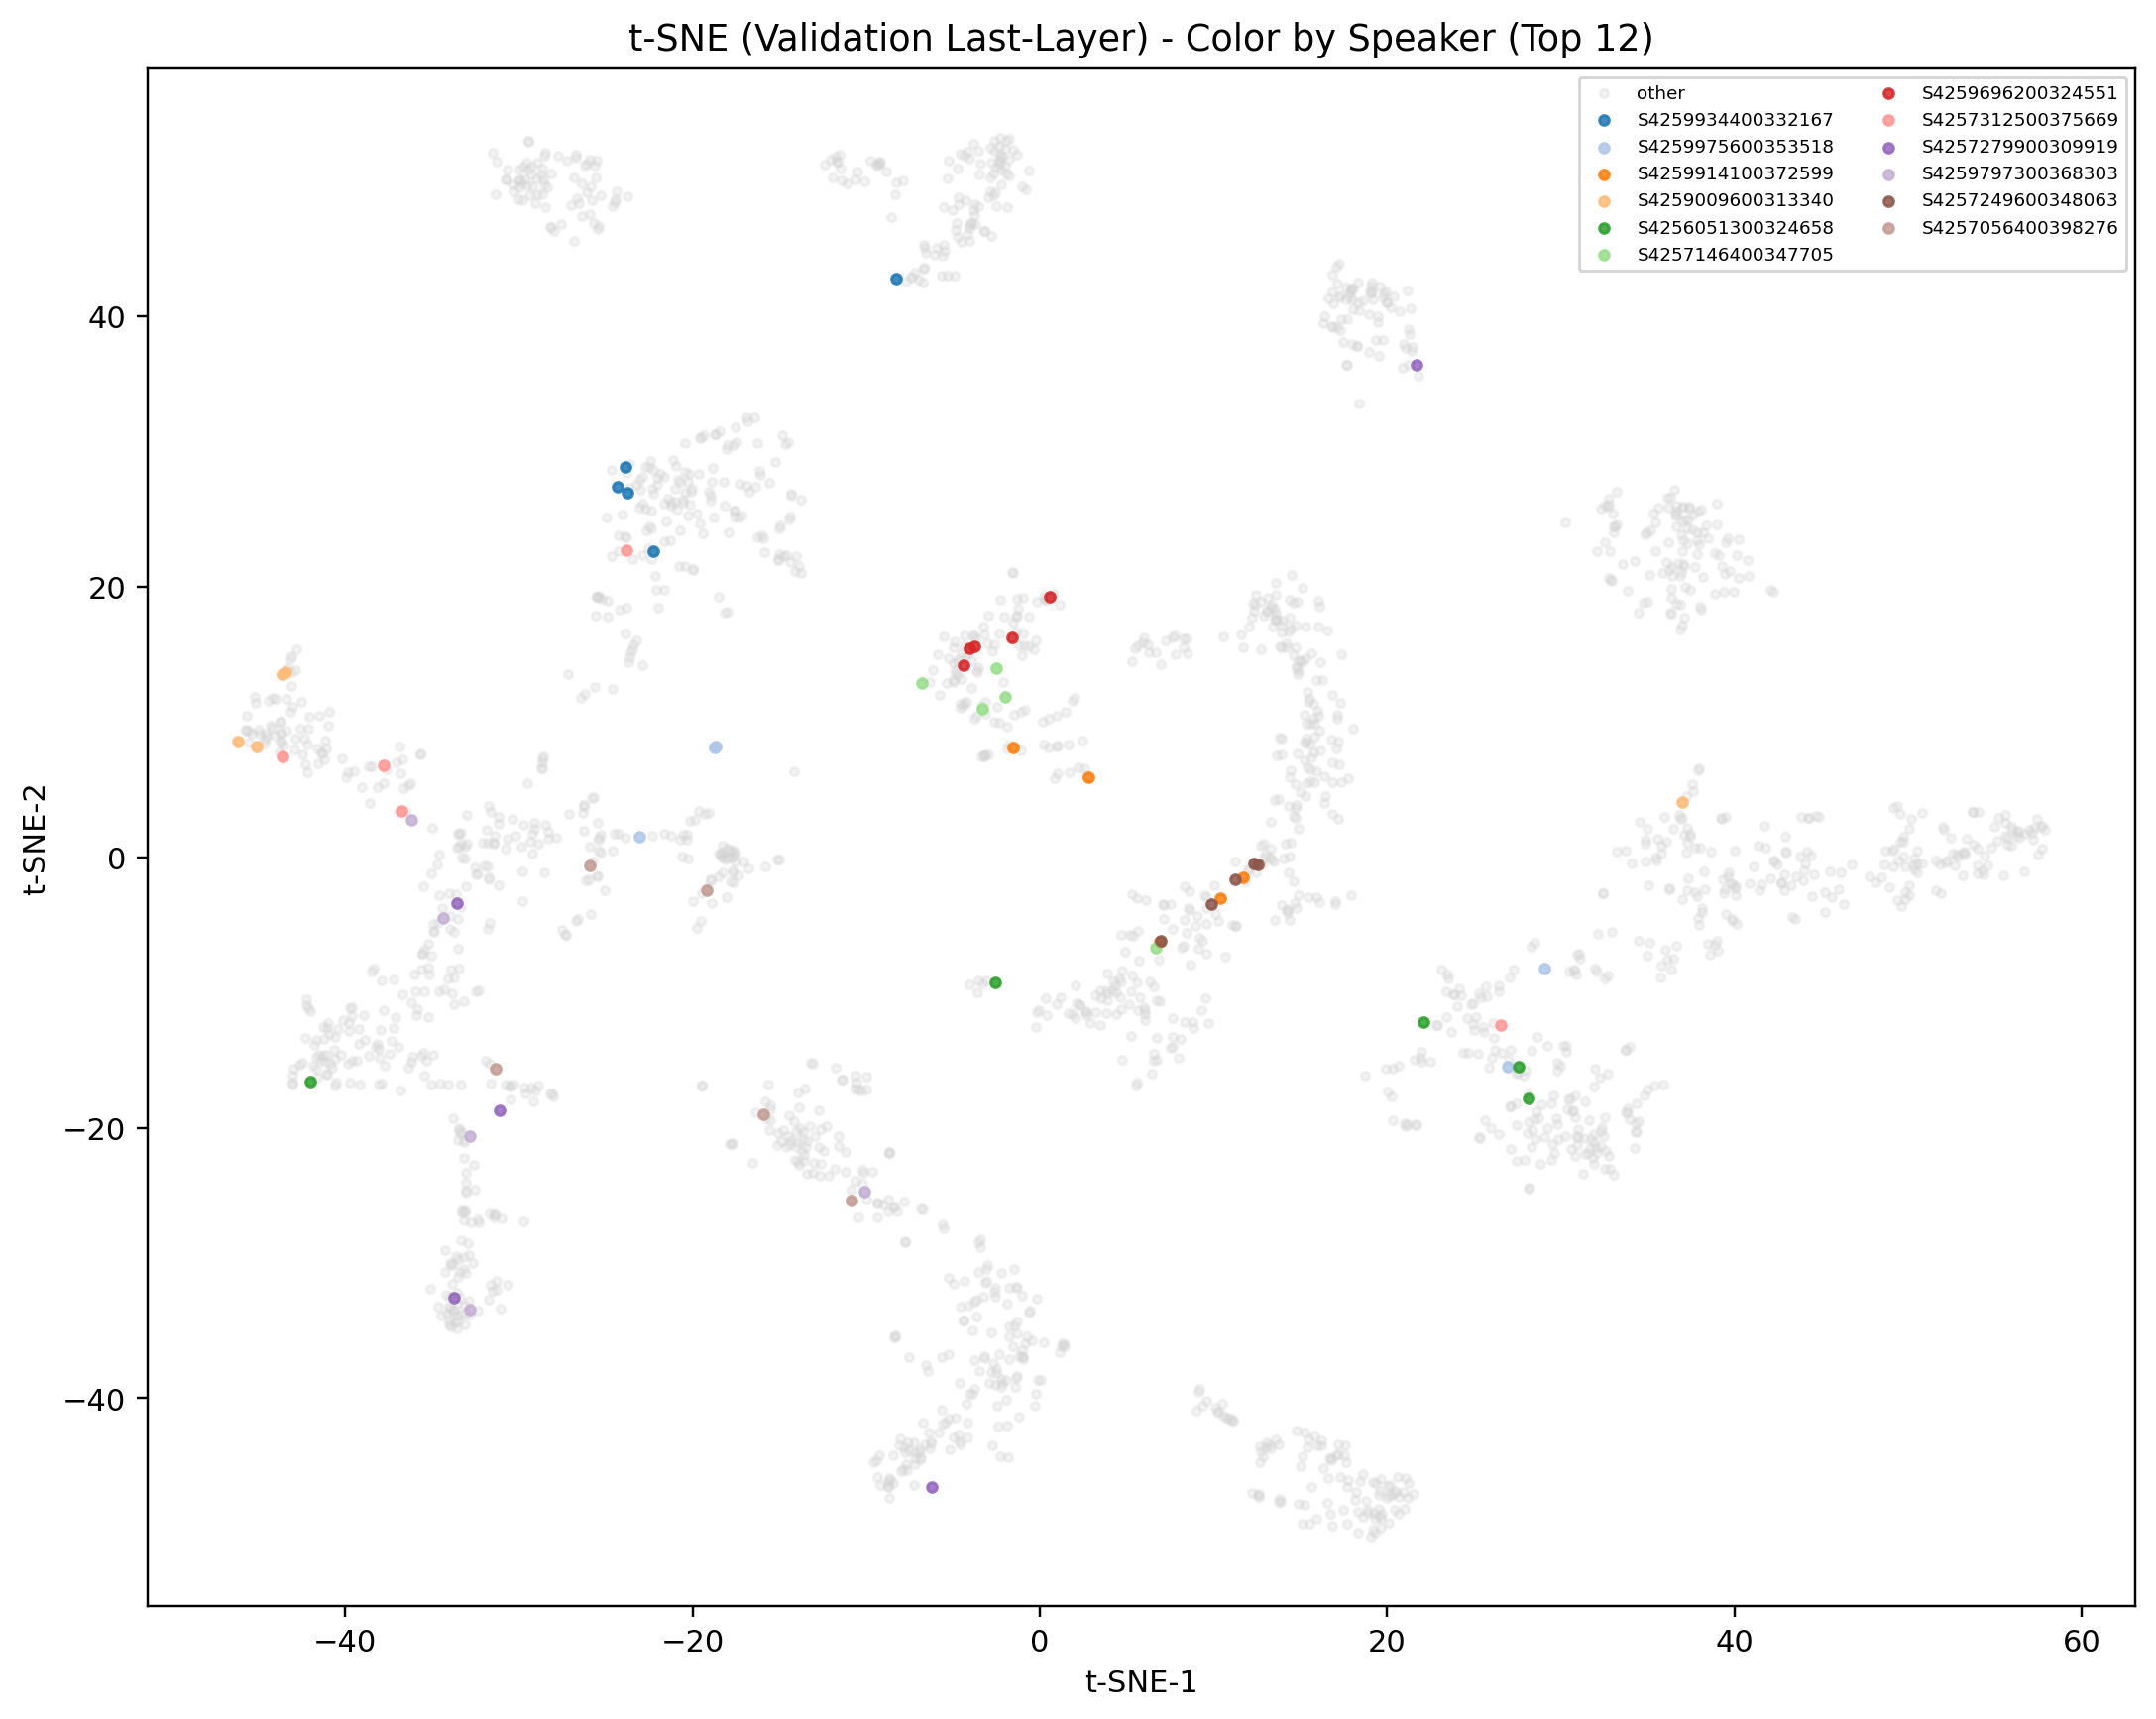
\includegraphics[width=0.48\linewidth]{figures/tsne_dann_by_speaker.png}
    \caption{DANN t-SNE on validation embeddings: by language (left), by speaker (right).}
    \label{fig:tsne_dann}
\end{figure}

\FloatBarrier

\section*{7 conclusion}
Tuned mHuBERT is a strong no-mitigation reference. Mitigation quality is configuration-sensitive: mild data-centric augmentation helps, while overly aggressive augmentation can hurt. The best final model is DANN, which gives the strongest overall performance and better weak-class recovery under strict unseen-speaker validation. Analysis confirms meaningful bias reduction, with remaining hard confusion pairs and residual speaker signal.

\renewcommand{\refname}{Reference}
\bibliographystyle{acl_natbib}
\bibliography{custom}

\end{document}
